% This is a model template for the solutions in computational science. You can find a very useful documentation for LaTeX in Finnish at ftp://ftp.funet.fi/pub/TeX/CTAN/info/lshort/finnish/ or in English at ftp://ftp.funet.fi/pub/TeX/CTAN/info/lshort/english/. The section List of mathematical symbols in Chapter 3 is especially useful for the typesetting of mathematical formulas.

% Compile the document to PDF by command 'pdflatex model.tex' in the terminal. The command must be run twice for the references in the text to be correct.

\documentclass[a4paper,11pt]{article}
\usepackage[utf8]{inputenc}
% This includes letters such as � and �
\usepackage[T1]{fontenc}
% Use here 'Finnish' for Finnish hyphenation. You may have to compile the code twice after the change. 
\usepackage[english]{babel}
\usepackage{graphicx}
% Some math stuff
\usepackage{amsmath,amsfonts,amssymb,amsbsy,commath,booktabs}  
% This is just to include the urls
\usepackage{hyperref}
\usepackage[margin=2cm]{geometry}

\setlength{\parindent}{0mm}
\setlength{\parskip}{1.0\baselineskip}

\usepackage{listings}
\usepackage{color}

\definecolor{dkgreen}{rgb}{0,0.6,0}
\definecolor{gray}{rgb}{0.5,0.5,0.5}
\definecolor{mauve}{rgb}{0.58,0,0.82}

\lstset{frame=tb,
	language=Python,
	aboveskip=3mm,
	belowskip=3mm,
	showstringspaces=false,
	columns=flexible,
	basicstyle={\small\ttfamily},
	numbers=none,
	numberstyle=\tiny\color{gray},
	keywordstyle=\color{blue},
	commentstyle=\color{dkgreen},
	stringstyle=\color{mauve},
	breaklines=true,
	breakatwhitespace=true,
	tabsize=4
}

\begin{document}

\title{Becs-114.1100 Computational Science -- exercise round 1} % Replace the exercise round number
\author{Kunal Ghosh, 546247} % Replace with your name and student number
\maketitle

\section{Solution to Question 1}\label{prob1}

In this question we have been asked to compute the approximate values of $\epsilon_t$ the truncation error and $\epsilon_r$ the round off error of the function $f(x) = sin(x)$ at $x=0.5$

The round off error $(\epsilon_r)$ is caused by the limited numerical precision of computers. i.e. if our computer is correct upto 6 significant digits then 5.000000 will be equal to 5.0000001 however these two numbers are not equal. Therefore there is clearly, a possibility of error in representing numbers with fixed precision.

The truncation error $(\epsilon_t)$ is caused when we try to use infinite series expansion (for example taylor series) in our computation and we limit the number of terms in the expansion. For the terms that are not included in the expansion, an error is introduced. for example the truncation error using Taylor's theorem is $-\frac{h}{6}f'''(\zeta)$

The total error $\epsilon$ is calculated by summing up truncation and round off errors.
\begin{equation}
\epsilon = \epsilon_t + \epsilon_r
\end{equation}

Specifically, we have been asked to analyse the $sin(x)$ function. assuming $\zeta = 0.5$ we get the truncation error as:
\begin{equation}
\epsilon_t = -\frac{h}{6}(-cos(0.5))
\label{eqn:et}
\end{equation}

Also, the approximate value of the first derivative of a function using central limit formula is:
\begin{equation}
f'(x) \approx \frac{f(x+h) - f(x-h)}{2h}
\end{equation}

Since we need to calculate the first derivative about $ x = 0.5 $ then the above equation becomes..

\begin{equation}
f'(x) \approx \frac{f(0.5+h) - f(0.5-h)}{2h}
\end{equation}

and the analytical first derivative of $sin(x)$, the function under consideration, is $cos(x)$. So the total error $\epsilon$is calculated as..

\begin{equation}
\epsilon \approx \abs{\frac{f(0.5+h) - f(0.5-h)}{2h} - cos(x)}
\label{eqn:fdash}
\end{equation}

and from \ref{eqn:fdash} and \ref{eqn:et} we get..

\begin{equation}
\epsilon_r = \epsilon - \epsilon_t
\label{eqn:er}
\end{equation}
which is also a function of $h$. Now we generate 25 (arbitrary, we could have chosen more) values of $h$ by the following update equation $h \leftarrow {h} / {4}$.

Plotting \ref{eqn:fdash} , \ref{eqn:et} and \ref{eqn:er} as a function of $h$ on the log scale gives us \ref{fig:solution1_fig}. We use the log scale because in that scale really small values are scaled up which helps us visualize the values better.

\begin{figure}[h]
\centering
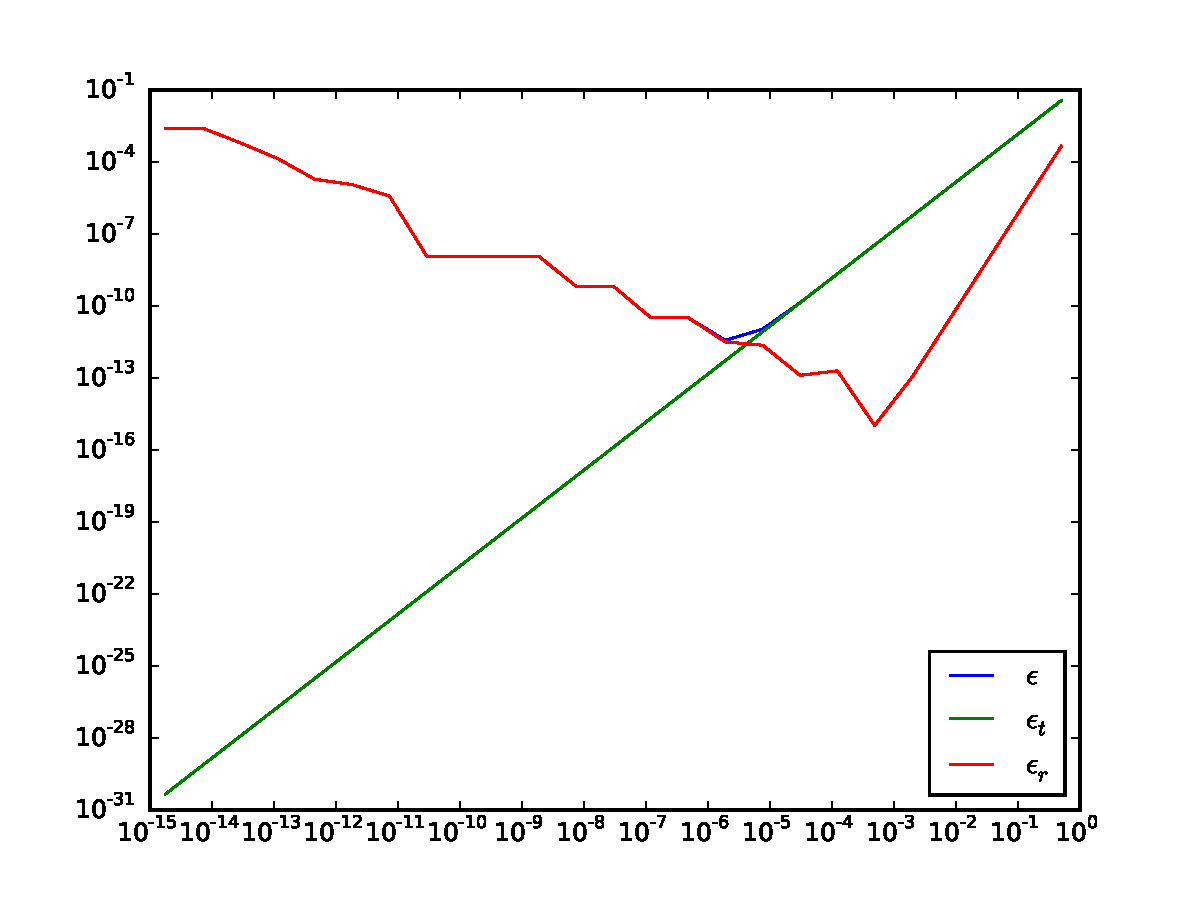
\includegraphics[scale=0.45]{solution1_fig}
\caption{Total, truncation and rounding errors for $sin(x)$ at $x = 0.5$.}
\label{fig:solution1_fig}
\end{figure}

The corresponding python code can be found at \ref{code:problem1}
\clearpage

\section{Solution to Question 3}\label{prob3}



\begin{figure}[h]
	\centering
	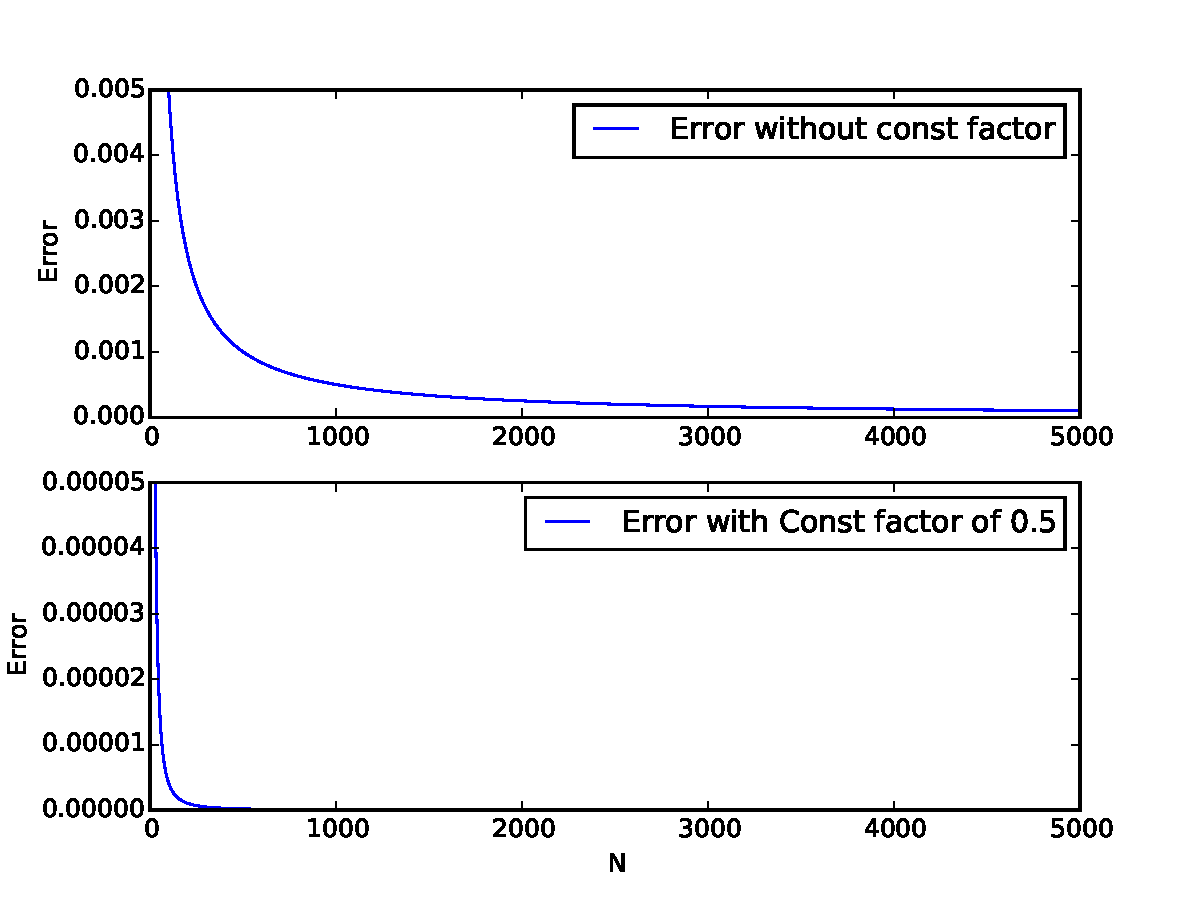
\includegraphics[scale=0.45]{figure_3.pdf}
	\caption{The error between analytical solution and taylor approximation. First row is for equation $(e^x - 1)/x$ and the second row for equation $(e^x - e^{-x}) / 2x$. The third column shows the graphs in the second column magnified at the point of inflexion.}
	\label{fig:solution3_fig}
\end{figure}

\begin{center}
	\begin{table}[h!]
	\begin{tabular}{|c|c|c|c|c|c|}
\hline
& Index & Approximation ln(n) & Error & Approx ln(n + 0.5) & Error \\
\hline
& 100 & 0.582207331652 & 0.00499166675 & 0.57721979014 & 4.12523895743e-06 \\
& 200 & 0.579713581573 & 0.00249791667188 & 0.577216701375 & 1.03647328931e-06 \\
& 300 & 0.578881405643 & 0.00166574074177 & 0.577216126324 & 4.61422707043e-07 \\
& 400 & 0.578465144069 & 0.00124947916699 & 0.577215924668 & 2.59766558375e-07 \\
& 500 & 0.578215331568 & 0.000999666666796 & 0.577215831235 & 1.66333712026e-07 \\
& 600 & 0.578048766753 & 0.000833101851918 & 0.57721578045 & 1.15548026147e-07 \\
& 700 & 0.577929780548 & 0.000714115646296 & 0.577215749814 & 8.49126385871e-08 \\
& 800 & 0.577840534693 & 0.000624869791689 & 0.577215729924 & 6.50228465515e-08 \\
& 900 & 0.577771117576 & 0.000555452674911 & 0.577215716285 & 5.13832113525e-08 \\
& 1000 & 0.577715581568 & 0.000499916666674 & 0.577215706527 & 4.16250224289e-08 \\
& 1100 & 0.577670141486 & 0.000454476584025 & 0.577215699306 & 3.44039702282e-08 \\
& 1200 & 0.577632273698 & 0.000416608796297 & 0.577215693813 & 2.89110814178e-08 \\
& 1300 & 0.577600230976 & 0.000384566074948 & 0.577215689537 & 2.46358701217e-08 \\
& 1400 & 0.577572765242 & 0.000357100340135 & 0.577215686145 & 2.12433216573e-08 \\
& 1500 & 0.577548961198 & 0.000333296296296 & 0.577215683408 & 1.8506176036e-08 \\
& 1600 & 0.577528132349 & 0.000312467447919 & 0.577215681167 & 1.62658729819e-08 \\
& 1700 & 0.577509753714 & 0.000294088811997 & 0.577215679311 & 1.44090542831e-08 \\
& 1800 & 0.577493416959 & 0.000277752057617 & 0.577215677754 & 1.28529425991e-08 \\
& 1900 & 0.577478799712 & 0.000263134810718 & 0.577215676437 & 1.15359471975e-08 \\
& 2000 & 0.577465644068 & 0.000249979166669 & 0.577215675313 & 1.04114609156e-08 \\
& 2100 & 0.577453741243 & 0.000238076341646 & 0.577215674345 & 9.44372391398e-09 \\
& 2200 & 0.577442920411 & 0.000227255509644 & 0.577215673506 & 8.60490512178e-09 \\
& 2300 & 0.577433040453 & 0.000217375551359 & 0.577215672775 & 7.87307719019e-09 \\
& 2400 & 0.577423983767 & 0.000208318865748 & 0.577215672132 & 7.23079007781e-09 \\
& 2500 & 0.577415651568 & 0.000199986666667 & 0.577215671566 & 6.66399990745e-09 \\
& 2600 & 0.577407960266 & 0.000192295364887 & 0.577215671063 & 6.16133355447e-09 \\
& 2700 & 0.577400838656 & 0.000185173753993 & 0.577215670615 & 5.7134669218e-09 \\
& 2800 & 0.577394225701 & 0.000178560799306 & 0.577215670214 & 5.3127137134e-09 \\
& 2900 & 0.577388068786 & 0.00017240388425 & 0.577215669854 & 4.95269592005e-09 \\
& 3000 & 0.577382322309 & 0.00016665740739 & 0.57721566953 & 4.62806759582e-09 \\
& 3100 & 0.577376946553 & 0.000161281651047 & 0.577215669236 & 4.33435054514e-09 \\
& 3200 & 0.577371906763 & 0.000156241861965 & 0.577215668969 & 4.06772471262e-09 \\
& 3300 & 0.577367172401 & 0.000151507499219 & 0.577215668726 & 3.82496601059e-09 \\
& 3400 & 0.577362716516 & 0.000147051614738 & 0.577215668505 & 3.60329799332e-09 \\
& 3500 & 0.577358515242 & 0.000142850340118 & 0.577215668302 & 3.4003705407e-09 \\
& 3600 & 0.57735454736 & 0.000138882458819 & 0.577215668116 & 3.2140982098e-09 \\
& 3700 & 0.577350793949 & 0.000135129047945 & 0.577215667944 & 3.04274017093e-09 \\
& 3800 & 0.577347238078 & 0.000131573176341 & 0.577215667786 & 2.88472257193e-09 \\
& 3900 & 0.577343864551 & 0.000128199649333 & 0.57721566764 & 2.73870248702e-09 \\
& 4000 & 0.577340659693 & 0.000124994791638 & 0.577215667505 & 2.6034862044e-09 \\
& 4100 & 0.577337611164 & 0.000121946262113 & 0.57721566738 & 2.47804521347e-09 \\
& 4200 & 0.577334707796 & 0.000119042894908 & 0.577215667263 & 2.36146646682e-09 \\
& 4300 & 0.577331939464 & 0.0001162745628 & 0.577215667154 & 2.25292040579e-09 \\
& 4400 & 0.577329296961 & 0.000113632059199 & 0.577215667053 & 2.15168582951e-09 \\
& 4500 & 0.577326771897 & 0.000111106995859 & 0.577215666959 & 2.05713035495e-09 \\
& 4600 & 0.577324356615 & 0.000108691713897 & 0.57721566687 & 1.96866778435e-09 \\
& 4700 & 0.577322044108 & 0.000106379206252 & 0.577215666787 & 1.88579540872e-09 \\
& 4800 & 0.577319827951 & 0.000104163049742 & 0.57721566671 & 1.80804604621e-09 \\
& 4900 & 0.577317702247 & 0.000102037345518 & 0.577215666637 & 1.73500225298e-09 \\
& 5000 & 0.577315661568 & 9.99966666332e-05 & 0.577215666568 & 1.66629987586e-09 \\
\hline
\end{tabular}
\caption{ Table logging the Euler value approximations every 100 iterations. The second and the third columns correspond to the convergence equation without the constant and the third and fourth and fifth are ones with a constant (0.5 in this case) }
\label{table:1}
\end{table}
\end{center}

The corresponding python code can be found at \ref{code:problem3}

\clearpage
%\ldots

\section{Solution to Question 5}\label{prob5}

In this problem we have to calculate the error in analytical values and approximate Taylor values of given functions arguments tend to zero. The taylor approximates are useful because as the value of arguments tend to zero the analytical functions would become really large since the argument is in the denominator.

Deriving the taylor approximate of $f_1(x) = \frac{e^x - 1}{x}$ upto the 4th term (arbitrarily chosen)
\begin{equation}
f_1(x) = \frac{1}{x} (e^x - 1)
\label{eqn:q5_1}
\end{equation}
From taylor's expansion
\begin{equation}
e^x = e^0 + \sum_{i=1}^{n-1} \frac{x^i}{i!} e^{(i)}(0) + \frac{x^n}{n!} e^{(n)}(\zeta)
\label{eqn:q5_2}
\end{equation}
substituting \ref{eqn:q5_2} (upto the 4th term i.e. n=4)in \ref{eqn:q5_1} and simplifying ( the $x$ in the denominator cancels out) we get.
\begin{equation}
\frac{1}{x} (e^x - 1) = \frac{1}{x} \left( \frac{x}{1!}e(0) + \frac{x^2}{2!}e^{2}(0) + \frac{x^3}{3!}e^{3}(0) + \frac{x^4}{4!}e^{4}(4) \right)
\end{equation}
\begin{equation}
\frac{1}{x} (e^x - 1) = 1 + \frac{x}{2} + \frac{x^2}{6} + \frac{x^3}{24}e^{4}
\label{eqn:q5_4}
\end{equation}

The approximate value of \ref{eqn:q5_1} is calculated using \ref{eqn:q5_4} for small values of $x$ and then the two are subtracted to get the error which is plotted in \ref{fig:solution5_fig}

Similarly for $f_2(x) = (e^x - e^{-x}) / 2x$ Deriving the taylor approximate upto the 4th term we get.
\begin{equation}
\frac{(e^x - e^{-x})}{2x}  = \frac{1}{2x} \left[ \left( \frac{x}{1!}e(0) + \frac{x^2}{2!}e^{2}(0) + \frac{x^3}{3!}e^{3}(0) + \frac{x^4}{4!}e^{4}(4) \right) 
-  \left( \frac{x}{1!}e(0) - \frac{x^2}{2!}e^{2}(0) - \frac{x^3}{3!}e^{3}(0) + \frac{x^4}{4!}e^{4}(4) \right) \right]
\label{eqn:q5_5}
\end{equation}

\begin{equation}
\frac{(e^x - e^{-x})}{2x}  = 1 + \frac{x^2}{3!}
\label{eqn:q5_6}
\end{equation}

As for the first function, approximate value of \ref{eqn:q5_5} is calculated using \ref{eqn:q5_6} for small values of $x$ and then the two are subtracted to get the error which is plotted in \ref{fig:solution5_fig}

\begin{figure}[h]
	\centering
	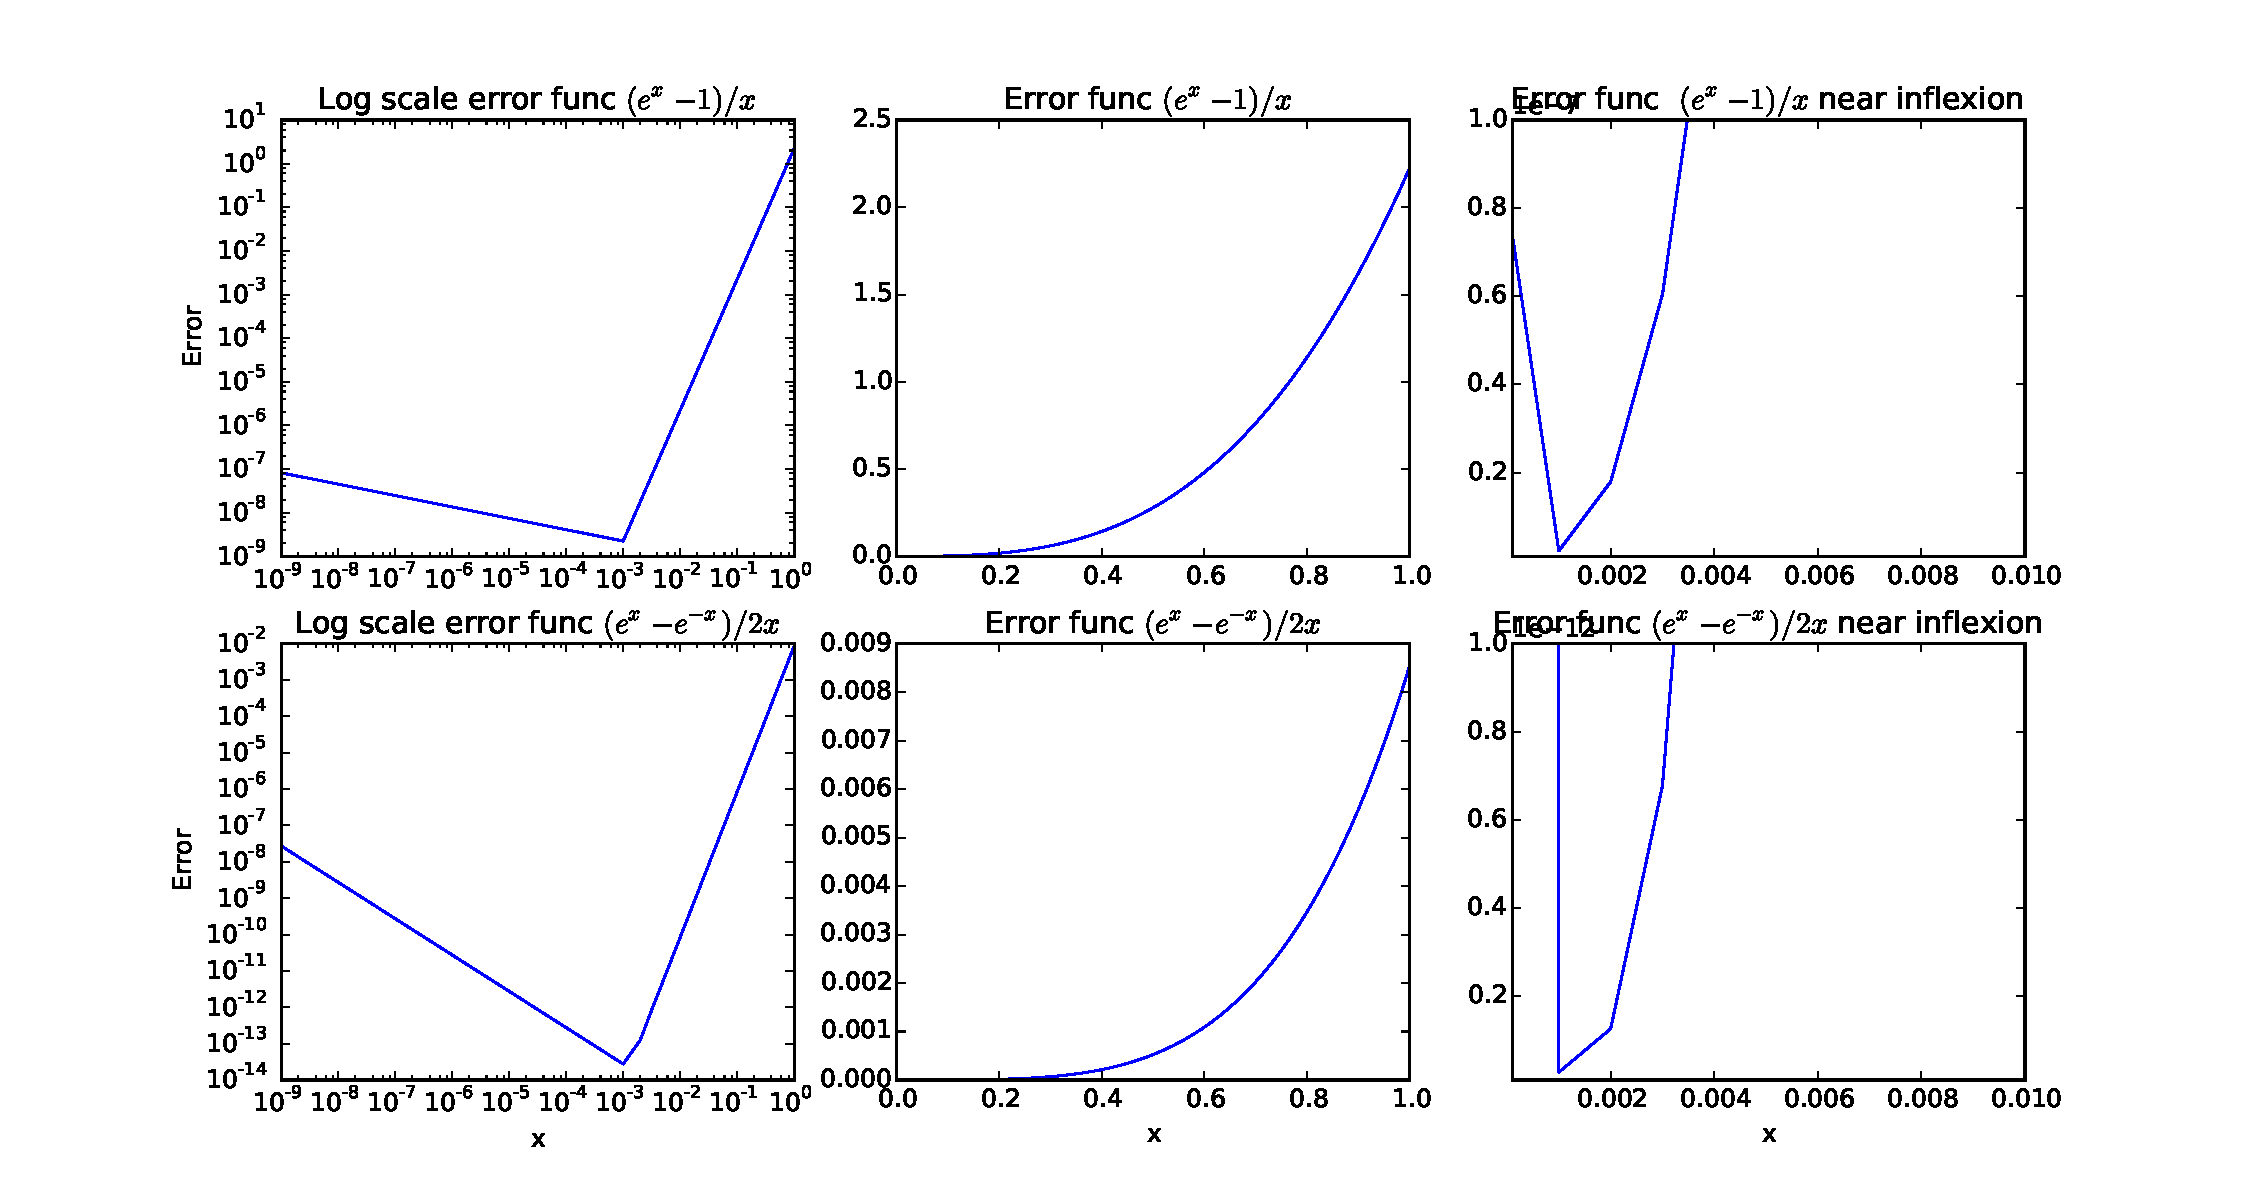
\includegraphics[scale=0.45]{solution_5_fig.pdf}
	\caption{}
	\label{fig:solution5_fig}
\end{figure}

The corresponding python code can be found at \ref{code:problem5}

\clearpage
\appendix

\section{Appendix A}\label{code:problem1}
Python source code for \ref{prob1}.
{\footnotesize
\begin{lstlisting}
from __future__ import division
import pylab as pl
import numpy as np
from numpy import sin,cos

def f_dash_central_diff(f,x,h):
	# Calculating the derivative of f at x with interval size h
	# using the central limit theorem
    return (f(x + h) - f(x - h)) / (2 * h)

def calculate_error_and_plot():
	# The value at which the function is to be evaluated.
    x = 0.5
    
    # Initial value of the step size
    h_initial = 0.5
    # Generate a list of values of h each obtained by dividing by a power of 4
    h = np.asarray([h_initial/(4 ** _) for _ in range(25)])

    # The function being evaluated
    f = sin
    # The analytical first derivative of sin(x)
    f_dash = cos
    # The analytical 3rd derivative of sin(x)
    f_3dash = lambda x: -1 * cos(x)

    # Total error
    error_total = abs(f_dash_central_diff(f,x,h) - f_dash(x))
    # Truncation error
    error_trunc = abs((-1 * (h ** 2)/6) * f_3dash(x))
    # Round off error
    error_round = abs(error_total - error_trunc)

    print(h, error_total,  error_trunc, error_round)
    # Plotting the values on the log scale
    pl.loglog(h, error_total, h, error_trunc, h, error_round)
    pl.legend(["$\epsilon$", "$\epsilon_t$", "$\epsilon_r$"], loc = 4)
    pl.savefig("solution1_fig.pdf")
    pl.show()

if __name__ == '__main__':
    calculate_error_and_plot()
\end{lstlisting}
}



\clearpage
\section{Appendix B}\label{code:problem3}
Python source code for \ref{prob3}.
{\footnotesize
\begin{lstlisting}
# Program to estimate the Euler's Constant.
# Print intermediate answers at every 100 steps
from __future__ import division
import math
import sys
import pylab as pl

Euler_Constant = 0.5772156649015329

running_sum_for_all_consts = {}
def print_stdout(index, approx1, error1, approx_with_const, error_with_const):
sys.stdout.write("{:>5} -- {:<20} {:<20} -- {:<20} {:<20}\n".format(index, approx1, error1,  approx_with_const, error_with_const))

def get_euler(n, const=0):
# This method returns the approximation
# of the euler's constant when considering a
# partial sum of n terms in the harmonic series
# Const : is used to speed up the convergence

running_sum = None
if const in running_sum_for_all_consts:
running_sum = running_sum_for_all_consts[const]
else:
running_sum_for_all_consts[const] = {}
running_sum = running_sum_for_all_consts[const]

harmonic_sum = 0
if n-1 in running_sum.keys():
# If we have calculated the sum of harmonic
# series till n-1 use that. (Memoization)
harmonic_sum = running_sum[n-1] + 1/n
running_sum[n] = harmonic_sum
else:
# usually happens for n=1
harmonic_sum = 1/n
running_sum[n] = harmonic_sum

euler_approx = harmonic_sum - math.log(n + const)
return euler_approx


steps = 5000


if __name__ == "__main__":
errors_without_const = []
errors_with_const = []
indices =  []
const = 0.5
print_stdout("Index","Approximation ln(n)", "Error","Approx ln(n + {})".format(const), "Error")
for i in xrange(steps+1):
# +1 because xrange(n) generates values from 0 to n-1
if i == 0:
# we only want to calculate i from 1 to n(steps in this case)
# using range(steps)[1:] is very memory inefficient for
# large values of "steps"
continue
approx_val = get_euler(i)
approx_val_const = get_euler(i,const)

indices.append(i)
errors_without_const.append(abs(approx_val - Euler_Constant))
errors_with_const.append(abs(approx_val_const - Euler_Constant))
if i % 100 == 0:
print_stdout(i, approx_val, errors_without_const[-1], approx_val_const, errors_with_const[-1])

pl.figure(1)
pl.subplot(211)
pl.plot(indices, errors_without_const)
pl.legend(["Error without const factor"], loc = 1)
pl.ylabel("Error")
pl.ylim(ymin=0,ymax=0.005)
# pl.xlim(xmin=0,xmax=200)
pl.subplot(212)
pl.plot(indices, errors_with_const)
pl.legend(["Error with Const factor of {}".format(const)], loc = 1)
pl.xlabel("N")
pl.ylabel("Error")
pl.ylim(ymin=0,ymax=0.00005)
# pl.xlim(xmin=0,xmax=50)
pl.savefig("figure_3.pdf")
pl.show()
\end{lstlisting}
}

\clearpage
\section{Appendix C}\label{code:problem5}
Python source code for \ref{prob5}.
{\footnotesize
\begin{lstlisting}

from __future__ import division
import numpy as np
import doctest
import pylab as pl

# Class encapsulating the first function
class function_1:
	@staticmethod
	def exact(x):
		# Exact analytical value
		'''
		>>> function_1.exact(1)
		1.718281828459045
		>>> function_1.exact(0.5)
		1.2974425414002564
		>>> function_1.exact(1/2)
		1.2974425414002564
		'''
		return ((np.e ** x) - 1) / x

	@staticmethod
	def taylor_approx(x):
		# Taylor approximation
		'''
		>>> function_1.taylor_approx(1)
		3.941589584714343
		>>> function_1.taylor_approx(0.5)
		1.5760320314226264
		>>> function_1.taylor_approx(1/2)
		1.5760320314226264
		>>> function_1.taylor_approx(0)
		1.0
		'''
		return 1 + (x/2) + ((x ** 2)/6) + ((x ** 3) * (np.e ** 4)/24)

# Class encapsulating the second function
class function_2:
	@staticmethod
	def exact(x):
		# Exact analytical value
		return ((np.e ** x) - (np.e ** (-1 * x))) / (2 * x)

	@staticmethod
	def taylor_approx(x):
		# Taylor approximation
		return 1 + ((x ** 2)/6)

if __name__ == "__main__":
	# Running the doc tests.
	doctest.testmod()
	
	#Generate 1000 values of x from 10^-9 to 1
	x = np.linspace(10 ** -9, 1, 1000)
	error_function1 = np.abs(function_1.taylor_approx(x) - function_1.exact(x))
	error_function2 = np.abs(function_2.taylor_approx(x) - function_2.exact(x))
	
	for index in xrange(len(error_function1)):
		print index, error_function1[index], error_function2[index]
	
	# Plot the first function
	pl.figure(1, figsize=(15,8))
	pl.subplot(231)
	pl.loglog(x,error_function1)
	pl.title("Log scale error func $(e^x - 1)/x$")
	pl.ylabel("Error")
	
	pl.subplot(232)
	pl.plot(x,error_function1)
	pl.title("Error func $(e^x - 1)/x$ ")
	
	pl.subplot(233)
	pl.plot(x,error_function1)
	pl.xlim(xmin=10**(-4), xmax=10**(-2))
	pl.ylim(ymin=10**(-9), ymax=10**(-7))
	pl.title("Error func  $(e^x - 1)/x$ near inflexion")
	
	# Plot the second function
	pl.subplot(234)
	pl.loglog(x, error_function2)
	pl.title("Log scale error func $(e^x - e^{-x}) / 2x$")
	pl.ylabel("Error")
	pl.xlabel("x")
	
	pl.subplot(235)
	pl.plot(x, error_function2)
	pl.title("Error func $(e^x - e^{-x}) / 2x$")
	pl.xlabel("x")
	
	pl.subplot(236)
	pl.plot(x, error_function2)
	pl.xlim(xmin=10**(-4), xmax=10**(-2))
	pl.ylim(ymin=10**(-14), ymax=10**(-12))
	pl.title("Error func $(e^x - e^{-x}) / 2x$ near inflexion")
	pl.xlabel("x")

	# Save the figure as a pdf
	pl.savefig("solution_5_fig.pdf")
	# Show the figure
	pl.show()

\end{lstlisting}
}

\end{document}
